\documentclass[DM,lsstdraft,SDP]{lsstdoc}
%Replace the CUx here and all \CU will resolve below.

\usepackage{gwp}
\usepackage{risk}

\begin{document}

\setDocTitle    [DM Charter\CU]
                    {\color[rgb]{0.16,0.42,0.57} \sf Data Management Organization Charter 
                    }
\setDocAuthor   {William O'Mullane, Marion Juric, Jeffrey P Kantor,  Tim Axelrod,  Roberta Allsman}                % the author(s) \setDocApprove  {LSST Project Oeefice}              % approval by ...
\setDocRef      {LDM-294} % the reference code
\setDocIssue    {2}                        % the issue
\setDocRevision {1}                        % the revision
\setDocDate     {\today}              % the date of the issue
\setDocStatus   {draft}                    % the document status

%
% a short abstract
%
\setDocAbstract {This is the DM plan updaed from the v2 of 2014.
   It covers the organisation anfd managemnt of DM for LSST.}

%
% the title page
%
\mktitle

%
%   Revision history
%
% MOST RECENT FIRST
\begin{docHistory}
\addtohist{2}{1}{2017-01-09}{WOM,MJ}{Update in TeX}
\addtohist{2}{0}{2015-03-11}{JK}{Updated with new RFC process, realignment of TCT, SAT, DMLT - other versions in between}
\addtohist{1}{1}{2004-06-23}{JK}{Initial version} 
\end{docHistory}

%
%   TOC
%
\newpage
\setcounter{tocdepth}{3}
\tableofcontents
\newpage

%
% It's all yours from here on
%


\frame{\frametitle{ A little about myself}
\begin{itemize}
\item 1985ish Life started with BASIC on a  commodore 
\item 1993 graduated  Computer Science Degree and Masters University College Cork, Ireland 
\item 1993 - 1997 Spacecraft Control Systems (C++) in ESA Mission Operations Centre Darmstadt Germany
\item 1997 - 2001 Hipparcos, Integral, Planck, Gaia, Bepi-Sax  (C,Java,Oracle, HTM, HEALPix) in ESA Technology Research Centre Noordwijk Netherlands
\item 2001-2003 Commercial programming - some Astronomy (Java) 
\item 2003-2005 The Johns Hopkins, SDSS and National Virtual Observatory (C,C\#,Java,Sqlserver)
\item 2005-2014 Gaia Astrometric Solution and Science Operations (Java, Oracle, Intersystems Cache) 
\item 2012  PhD in Physics on Implementing the Gaia Astrometric Solution,  Barcelona University
\item 2014-2017 All ESA Science Ground Segments in Development
\end{itemize}
}

\frame{\frametitle{Induction to astronomy : HIP Catalogue}
1997/98 Hipparcos Java Tools - learning Astrometry
\url{http://www.cosmos.esa.int/web/hipparcos/java-tools}
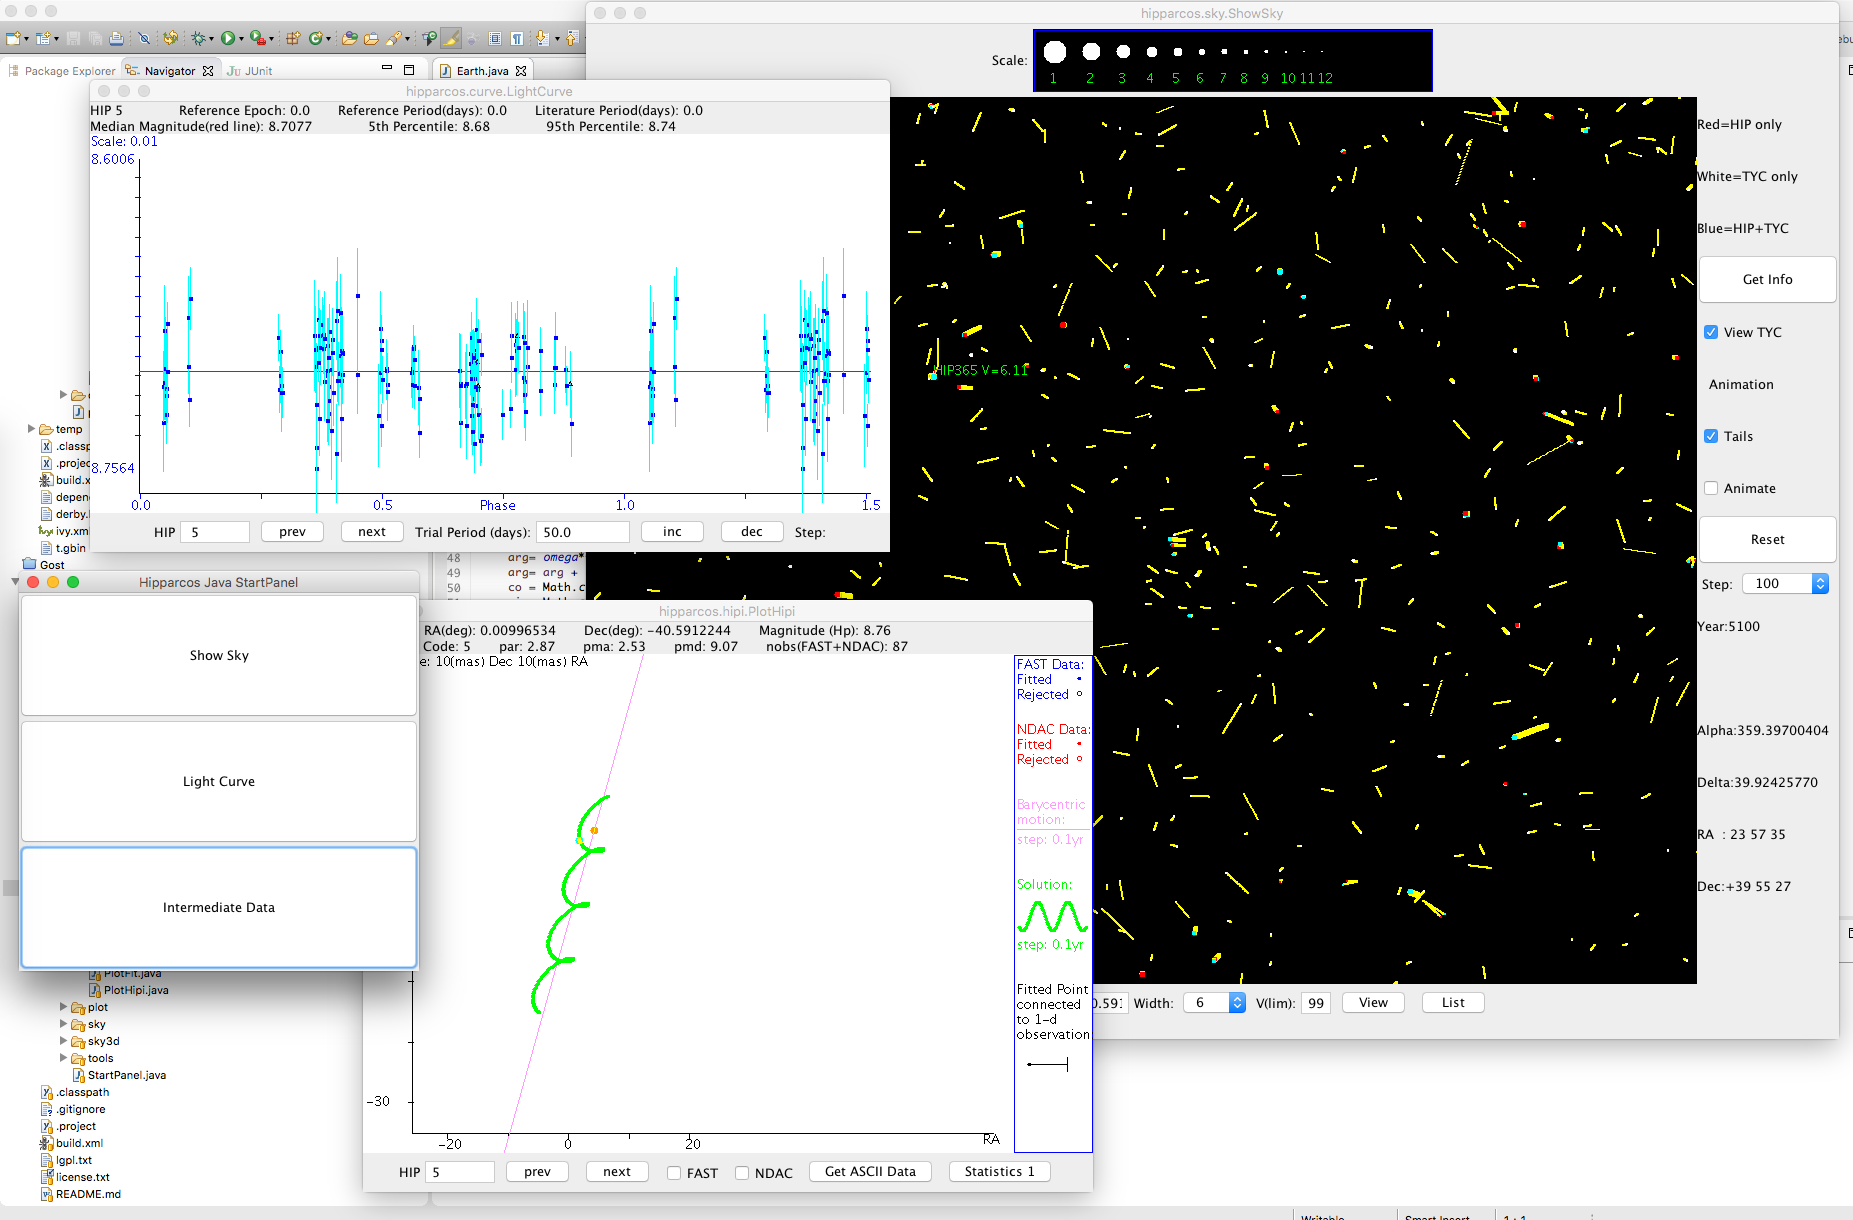
\includegraphics[width=\textwidth]{hipjt}
}

\frame{\frametitle{In the USA .. }
\vspace{5pt}
\begin{columns}[c]
\column{0.6\textwidth}
\vspace{4pt}
Quality tools for GSC2 (Java) $\rightarrow$\\
\vspace{8pt}
CasJobs (C\#)\citep{conf:casjobs}
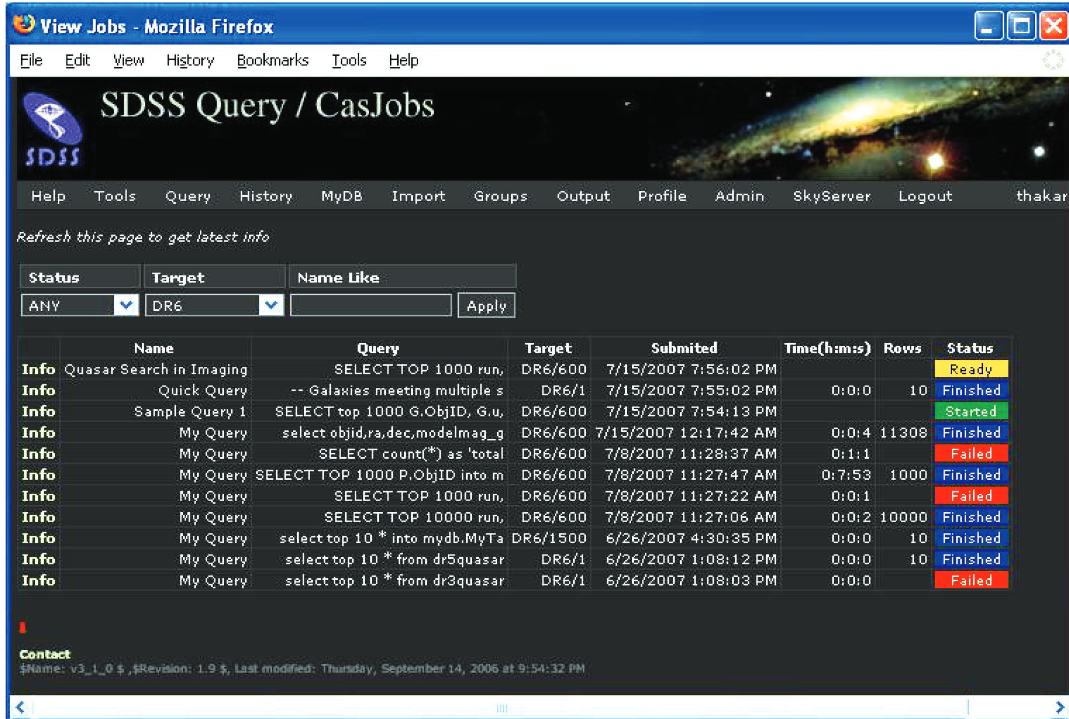
\includegraphics[width=\textwidth]{casjobs}
\column{0.4\textwidth}
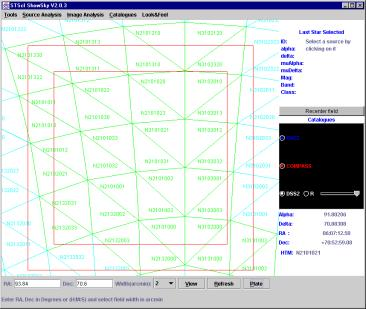
\includegraphics[width=\textwidth]{sshtm}
\vspace{-1cm}
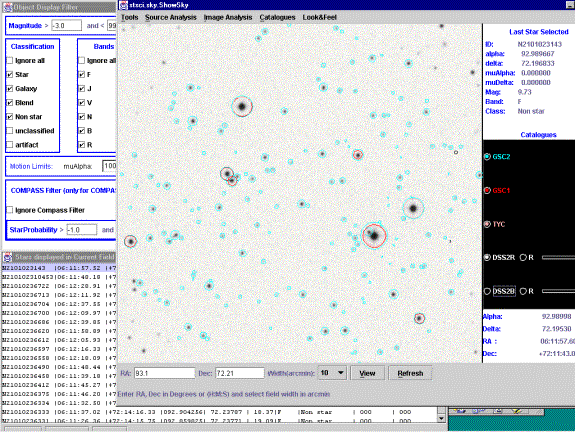
\includegraphics[width=\textwidth]{showsky}
\end{columns}
}


\frame{\frametitle{European Space Astronomy Centre }
\begin{columns}[c]
\column{0.4\textwidth}

\includegraphics[width=0.9\textwidth]{exm}\\

\includegraphics[width=0.45\textwidth]{bepiclogo}
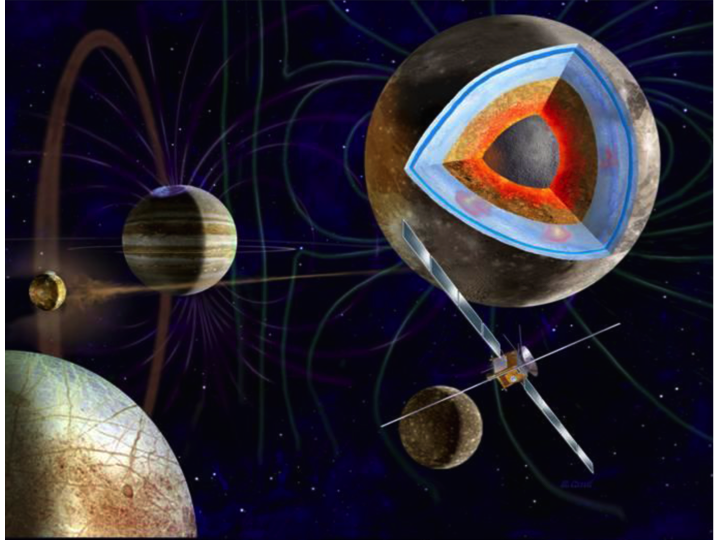
\includegraphics[width=0.45\textwidth]{juice}\\
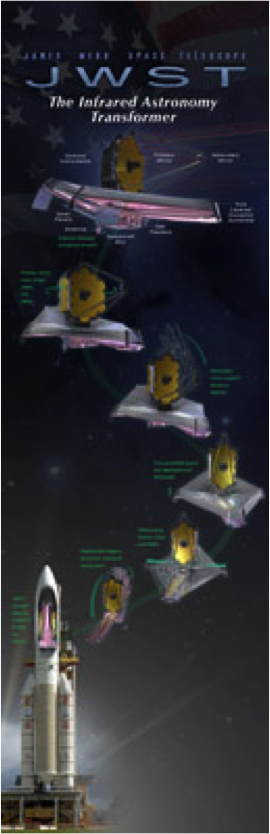
\includegraphics[width=0.45\textwidth]{jwst}\\
\vspace{-6cm}
\hspace{2.2cm}
\includegraphics[width=0.45\textwidth]{solo}\\
\hspace{2.2cm}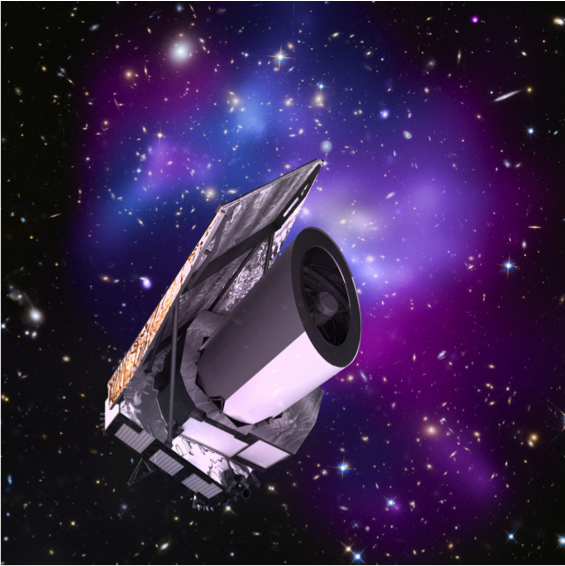
\includegraphics[width=0.45\textwidth]{euclid}

\column{0.6\textwidth}
\begin{itemize}
\item ESAC Located near Madrid, Spain.
\item Home of the Science Operations Department  containing  Operations Development Division.
\item Develop Science Operations Systems:
\begin{itemize}
\item People, Procedures and Software.
\item Interactions MOC and scientific communities.
\item Quite a bit of software - diverse - mainly Java but FORTRAN, C, C++, Python ..
\item Prepare for planning, simulations, instrument performance, commanding.
\item Hand over system to operations division after commissioning.

\end{itemize}
\end{itemize}
\end{columns}
}




\frame {\frametitle{ Data management }
    \begin{itemize}
	\item Victor remains interim PM until April 
	\item Have been trying to get an idea of DM organisation - talking to DMLT and TCAMS 
	\item Following are some observations and draft ideas 

    \end{itemize}

    {\bf   Look out for a  new version of LDM-294 - DM Management Plan}
    \begin{itemize}
	\item It will detail roles and responsibilities in DM
    \end{itemize}
    \vspace{12pt}
    DM Mission :\\
    {\em  Stand up operable, maintainable, quality services to deliver high-quality LSST data products for sciencer, all on time and within reasonable cost.}
}


\frame {\frametitle{ DM Organisation}

      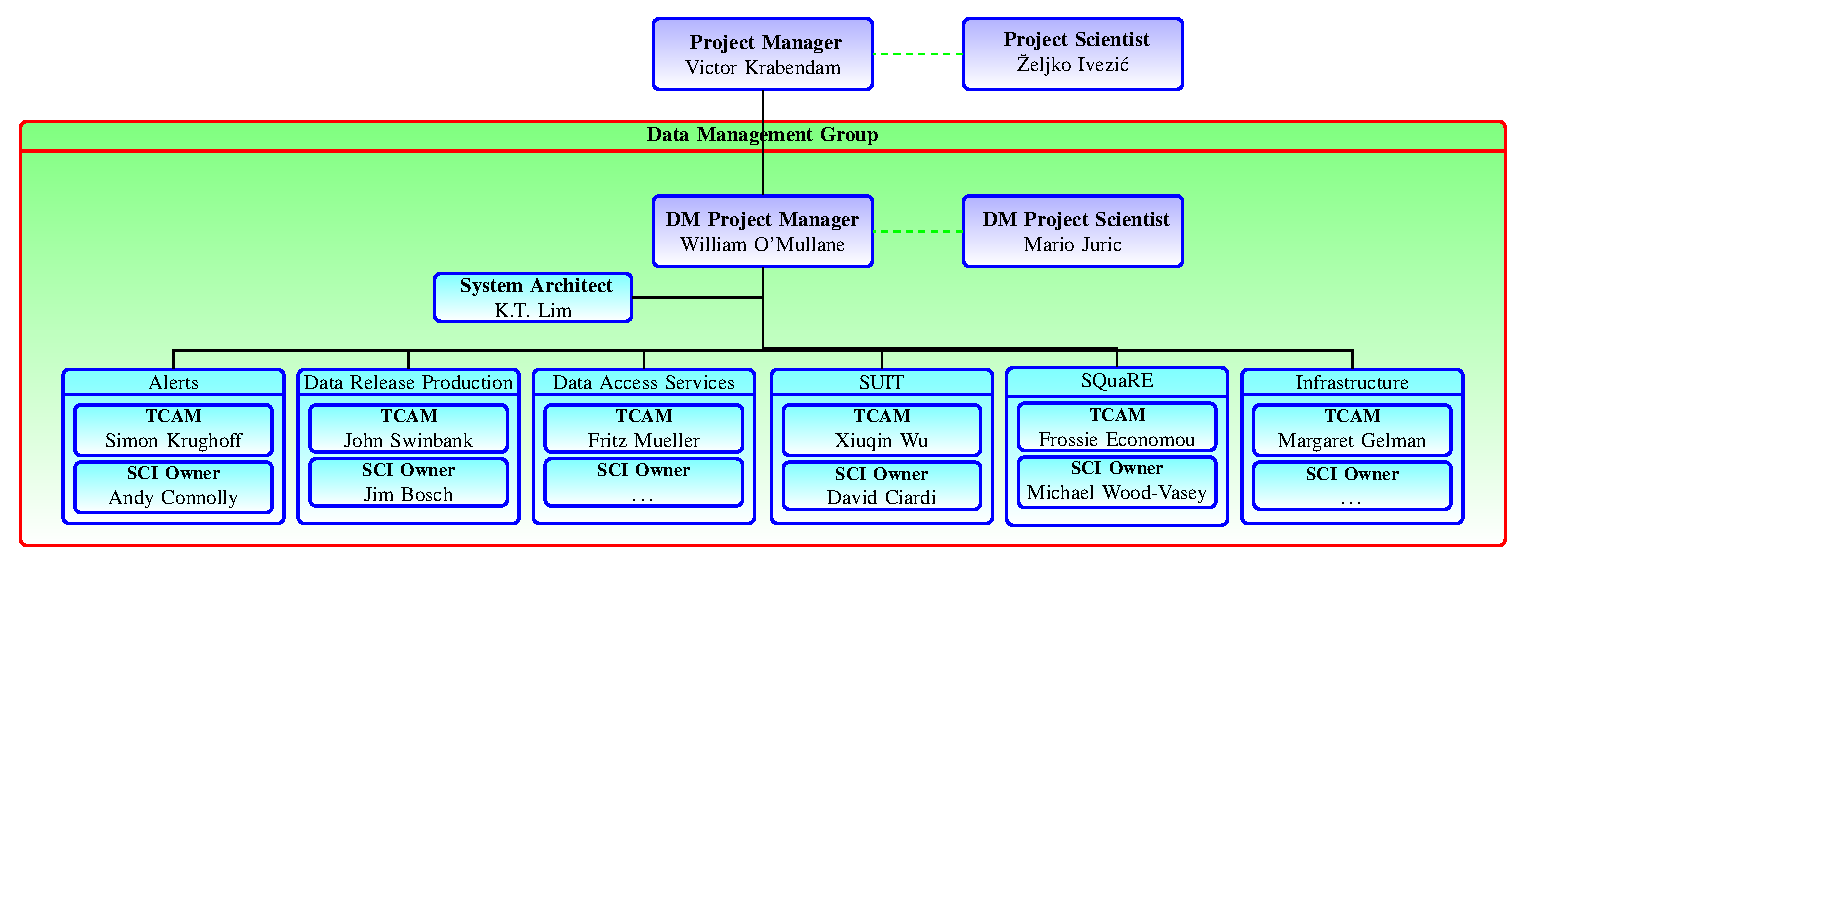
\includegraphics[width=1.0\textwidth]{images/DmOrg}\\
}

\frame {\frametitle{ DM architecture \& products}
	\begin{itemize}
	\item Would like to get  a list of products in DM
	\item Related to understanding the DM architecture - KT working on LDM-148 update more from him in a while
	\item Those are not Data Products - mostly Systems and Software artefacts
	\item For each product identify {\em Product Owner} and manager.
	\item This would change the org chart ..
	
	\end{itemize}

}

\frame {\frametitle{ Risk Management and other processes ..}
Also in LDM-294:
	\begin{itemize}
	 \item Would like an open Risk approach - anyone can raise a risk (Tim working on that)	
	 \item Document management - in next slid as
	 \item Configuration control 
	 \item Product assurance  and Scientific Validation 
	\item \ldots
	\end{itemize}
Mainly these will be high level and point to the details in other documents. 

}


\end{document}
